\documentclass[11pt]{article}
\usepackage[a4paper,margin=22mm]{geometry}
\usepackage{amsmath,amssymb,booktabs,longtable,array,enumitem,graphicx,xcolor}
\usepackage[hidelinks]{hyperref}
\usepackage{tikz}
\usetikzlibrary{arrows.meta,positioning,calc,shapes.geometric}
\setlength{\parindent}{0pt}
\setlength{\parskip}{6pt}
\setlist[itemize]{nosep}
\setlist[enumerate]{itemsep=3pt}
\newcommand{\sol}{\paragraph{Solution.}}
\newcommand{\SA}{\mathrm{SA}}
\newcommand{\up}{\mathord{\Uparrow}}
\newcommand{\dn}{\mathord{\Downarrow}}
\newcommand{\any}{\mathord{\Updownarrow}}
\hypersetup{pdftitle={VLSI Testing: rebuilt examination and independent solutions},pdfauthor={}}
\begin{document}
\title{VLSI Testing: 2013 Final}\author{}\date{}\maketitle\begin{quote}\small
Reconstructed questions and independently derived solutions. Personal names, identifiers,
handwritten answers and administrative headers are omitted. Figures are redrawn as
logical diagrams or explicit netlists. A source-reading note identifies a meaningful
ambiguity instead of silently changing the question. Finite Boolean checks
are supplied in the examination collection's Python verification script.
\end{quote}

\section{Full-scan conversion and stuck-at tests}
\textbf{Question.} Convert the sequential circuit to full scan, derive tests
covering all stuck-at faults of the combinational logic, and describe the
application sequence. The reconstructed normal-mode netlist is:
\begin{center}\begin{tabular}{ll}\toprule Signal & Defining expression\\\midrule
$g_1$ & $\overline{X_2\oplus Q_1}$\\
$g_2$ & $\overline{g_1\oplus Q_2}$\\
$h$ & $g_2\oplus Q_3$\\
$Y$ & $\overline{X_1+h+Q_4}$\\
$D_1$ & $g_2$\\
$D_2$ & $Q_1$\\
$D_3$ & $g_1$\\
$D_4$ & $Q_3$\\
\bottomrule\end{tabular}\end{center}
\begin{center}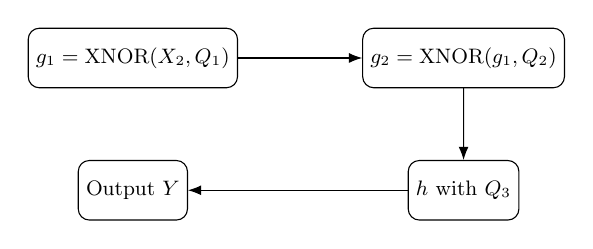
\begin{tikzpicture}[>=Latex,box/.style={draw,rounded corners,align=center,minimum height=9mm,font=\small},scale=0.84,transform shape]
\node[box] (g1) at (0,0) {$g_1=\operatorname{XNOR}(X_2,Q_1)$};
\node[box] (g2) at (5,0) {$g_2=\operatorname{XNOR}(g_1,Q_2)$};
\node[box] (h) at (5,-2) {$h$ with $Q_3$};
\node[box] (y) at (0,-2) {Output $Y$};
\draw[->] (g1) -- (g2);
\draw[->] (g2) -- (h);
\draw[->] (h) -- (y);
\end{tikzpicture}\end{center}

\sol Replace every D flip-flop by a muxed scan flip-flop:
$D_i^{\rm scan}=SE?SI_i:D_i$.
Connect $SI\to FF_1\to FF_2\to\cdots\to FF_n\to SO$ with common scan enable
and a controllable clock. Scan state outputs are independent pseudo-inputs;
all functional D inputs become observable pseudo-outputs.
\begin{center}\begin{tabular}{lll}\toprule $(X_1,X_2,Q_1,\ldots,Q_n)$ & $(D_1,\ldots,D_n)$ & $Y$\\\midrule
000000 & 0010 & 1\\
001011 & 1101 & 0\\
010110 & 0001 & 0\\
100000 & 0010 & 0\\
000100 & 1010 & 0\\
\bottomrule\end{tabular}\end{center}
Exhaustive enumeration of all $2^{6}$ input assignments verifies
54/54 single stuck-at faults for this netlist:
both values on every signal stem and on every individual gate-input branch.
Identity buffers at the observed D pins also model their separate output branches.
No modeled faults are redundant. The displayed set is sufficient, not claimed minimum.

For each row: assert $SE=1$; shift $Q_n,\ldots,Q_1$ in that order;
set $X_1,X_2$; deassert $SE$ and observe $Y$ before the capture edge;
apply one functional capture clock; reassert $SE$ and unload
$D_n,\ldots,D_1$ while loading the next state.
Account for scan-in/out bit order and compare only the expected response positions.
The proof covers combinational SAFs, not all scan-mux, clock, reset or analog defects.

\section{LFSR quotient stream and signature}
\textbf{Question.} Compute the quotient and final signature for two six-stage
LFSRs, feeding the rightmost input bit first, for
\[
M=\texttt{10000111011001001110101}.
\]
The first circuit distributes the last-stage feedback into XOR taps;
the second XORs selected register outputs into the serial input.
\begin{center}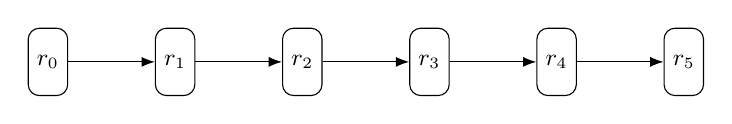
\begin{tikzpicture}[>=Latex,box/.style={draw,rounded corners,align=center,minimum height=9mm,font=\small},scale=0.95,transform shape]
\node[box] (r0) at (0.0,0) {$r_0$};
\node[box] (r1) at (1.7,0) {$r_1$};
\node[box] (r2) at (3.4,0) {$r_2$};
\node[box] (r3) at (5.1,0) {$r_3$};
\node[box] (r4) at (6.8,0) {$r_4$};
\node[box] (r5) at (8.5,0) {$r_5$};
\draw[->] (r0) -- (r1);
\draw[->] (r1) -- (r2);
\draw[->] (r2) -- (r3);
\draw[->] (r3) -- (r4);
\draw[->] (r4) -- (r5);
\end{tikzpicture}\end{center}

\sol The drawing does not state a seed, so assume a cleared register.
Number stages $r_0,\ldots,r_5$ from input to output and read the outgoing
$r_5$ \emph{before} each shift. No extra flush clocks are applied.
All sums below are XORs over $\mathrm{GF}(2)$.

For the distributed-feedback circuit, let $f=r_5$.
First form $(r_0',\ldots,r_5')=(u,r_0,r_1,r_2,r_3,r_4)$,
then XOR $f$ into positions $\{0,2,4,5\}$.
For the input-feedback circuit,
\[
r_0'=u+r_0+r_1+r_3+r_5,\qquad r_i'=r_{i-1}\quad(1\le i\le5).
\]
These recurrences, rather than a visually reversed polynomial label, define
the bit ordering unambiguously.
\begin{center}\begin{tabular}{lll}\toprule
Circuit & Serial output, first bit first & Final $(r_0,\ldots,r_5)$\\\midrule
Distributed & \texttt{00000011101111011010001} & \texttt{001000}\\
Input feedback & \texttt{00000011101111011010001} & \texttt{011000}\\
\bottomrule\end{tabular}\end{center}
The first six outgoing bits are the initial zero state.
Deleting that six-bit latency gives the emitted quotient portion during the
remaining input clocks. The table gives physical register signatures;
Fibonacci and distributed-feedback state encodings differ although their
outgoing streams agree. Reversing the signature, clocking six extra zeros or
using a nonzero seed changes the printed result and must be stated.

\section{Validity of March sequences}
\textbf{Question.} Which sequences have consistent read expectations on a
fault-free memory?
\begin{align*}
a&:\{\up(w0);\up(r0,w1);\dn(r0,w0,r0)\},\\
b&:\{\up(w0);\up(r1,w1);\dn(r1,w0,r0)\},\\
c&:\{\up(w1);\up(r1,w1);\dn(r1,w0,r0)\},\\
d&:\{\up(w1);\up(r1,w0);\dn(r0,w1,r1)\}.
\end{align*}
\sol Only $c,d$ are consistent.
In $a$, the second element leaves 1 in every cell, contradicting the next $r0$.
In $b$, the first $r1$ follows an initialization to 0.
In $c$, each descending visit reads 1, writes 0 and reads 0.
In $d$, the ascending pass leaves 0; the descending pass reads 0, writes 1,
then reads 1. Consistency does not itself imply completeness for any fault model.

\section{Equal SAF and transition-fault coverage}
\textbf{Question.} Compare
\begin{align*}
a&:\{\up(w0);\up(r0,w1);\dn(r1,w0)\},\\
b&:\{\up(w1);\up(r1,w0);\dn(r0,w1,r1)\},\\
c&:\{\up(w0);\up(r0,w1);\dn(r1,w0,r0)\}.
\end{align*}
\sol $b$ and $c$ both detect SA0, SA1, failed $0\to1$ transitions and
failed $1\to0$ transitions. They are data-complement versions of one another.
In $a$, $0\to1$ is read in the last element, but the final $1\to0$ is not
followed by a read, so a failed falling transition can escape.
The initialization and first read in each case also expose both stuck values.

\section{IEEE 1149.1 interconnect testing}
\textbf{Question.} Three ICs form the serial chain
$TDI\to IC1\to IC2\to IC3\to TDO$.
The four lines $X_1,\ldots,X_4$ run from IC1 outputs to IC2 inputs.
The course-specific instruction encodings are
Bypass=000, InTest=001 and ExTest=010.
The question requests driving 0000 to detect SA0 on $X_1,\ldots,X_4$.\begin{center}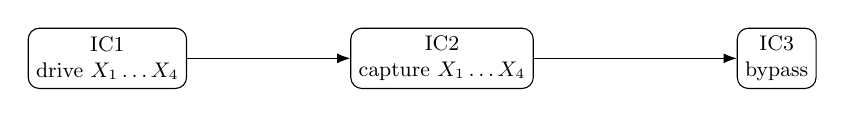
\begin{tikzpicture}[>=Latex,box/.style={draw,rounded corners,align=center,minimum height=9mm,font=\small},scale=0.85,transform shape]
\node[box] (i1) at (0,0) {IC1\\drive $X_1\ldots X_4$};
\node[box] (i2) at (5,0) {IC2\\capture $X_1\ldots X_4$};
\node[box] (i3) at (10,0) {IC3\\bypass};
\draw[->] (i1) -- (i2);
\draw[->] (i2) -- (i3);
\end{tikzpicture}\end{center}

\sol Put IC1 and IC2 in EXTEST; put the uninvolved IC3 in BYPASS.
Preload safe drive values, update the launch cells, allow interconnect settling,
capture at IC2, then shift out the captured response. Drive 1111 to detect SA0;
drive 0000 to detect SA1. Other boundary cells must have safe values, especially
output enables, to prevent contention.

\textbf{Correction to the printed request.} A line driven to 0 has the same
value under SA0, so 0000 cannot detect any of the four SA0 faults.
Use 1111 for the stated fault target; retain 0000 for SA1.
The hypothetical three-bit course encoding is used here, even though it is not
a universal device opcode assignment.

All three instruction registers have the stipulated length three.
Since the farthest IC's instruction is shifted first and each instruction is
LSB-first, load TDI bits
\[
\underbrace{000}_{IC3:\ Bypass}
\ \underbrace{010}_{IC2:\ ExTest}
\ \underbrace{010}_{IC1:\ ExTest}.
\]
From Run-Test/Idle, the TMS sequence 1100 reaches Shift-IR.
During the nine instruction shifts use eight zeros and a final 1, then 1,0
to reach Update-IR and return to Idle.
From Idle, 100 reaches Shift-DR via Capture-DR.
For a data register chain of length $L$, shift $L-1$ clocks with TMS=0 and the
last with TMS=1; then use 1,0 for Update-DR and Idle.
For response capture, take Idle$\to$Select-DR$\to$Capture-DR and then Shift-DR.

The figure does not specify serial ordering of the individual boundary cells,
their enable values or a BSDL description. Therefore the full TDI data word
cannot be uniquely inferred: it must encode 1111 at the four IC1 launch positions,
safe values elsewhere, and one IC3 bypass bit. If each depicted IC has exactly
eight boundary cells, $L=8+8+1=17$; use the actual BSDL lengths/order in hardware.
No assumption of arbitrary serial ordering should be hidden in a 17-bit answer.

\paragraph{Reset without TRST.}
Hold TMS=1 for at least five rising TCK edges, reaching Test-Logic-Reset
from any TAP state. A subsequent TMS=0 enters Run-Test/Idle.

\paragraph{1149.1 versus 1500.}
IEEE 1149.1 primarily gives chip/board boundary access through a TAP controller
and a standardized serial state machine. IEEE 1500 wraps embedded cores inside
an SoC; it separates the wrapper from the system-level test access mechanism
and supports wrapper serial access with optional parallel access for bandwidth.
Thus their intended integration level and access/control architecture differ.
See the TI boundary-scan design note and IEEE 1500 standard overview linked in
\texttt{exams/README.md}.

\section{Two wrapped cores and a three-bit TAM}
\textbf{Question.} Two IEEE 1500-wrapped cores are connected by a
three-bit daisy-chain TAM. The user-defined logic (UDL) is two two-input XORs
feeding a third XOR. Instructions are Bypass, InTest and ExTest.
(a) Generate tests for all UDL stuck-at faults.
(b) Give the serial external-test data path and procedure.
(c) Organize internal scan chains of lengths 120, 240, 240 and 120 to minimize
scan time, with the same operating frequency and supply for both cores.
\begin{center}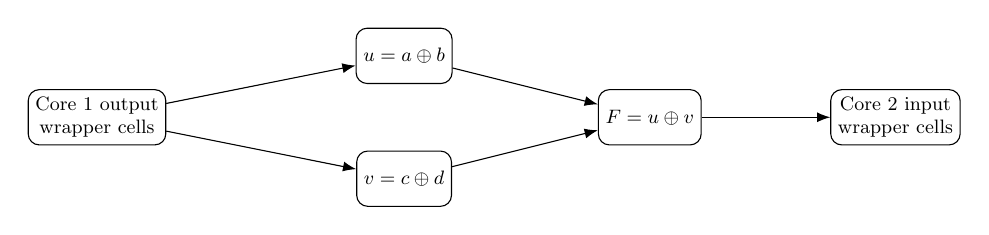
\begin{tikzpicture}[>=Latex,box/.style={draw,rounded corners,align=center,minimum height=9mm,font=\small},scale=0.78,transform shape]
\node[box] (c1) at (0,0) {Core 1 output\\wrapper cells};
\node[box] (a) at (5,1) {$u=a\oplus b$};
\node[box] (b) at (5,-1) {$v=c\oplus d$};
\node[box] (f) at (9,0) {$F=u\oplus v$};
\node[box] (c2) at (13,0) {Core 2 input\\wrapper cells};
\draw[->] (c1) -- (a);
\draw[->] (c1) -- (b);
\draw[->] (a) -- (f);
\draw[->] (b) -- (f);
\draw[->] (f) -- (c2);
\end{tikzpicture}\end{center}

\sol (a) Use $(a,b,c,d)\in\{0000,1000,0010,1111\}$.
Every primary input takes both values; each first-level XOR takes both values;
and the last XOR takes both values. Any single stuck-at error at a stem or
gate-input branch propagates through XORs without a controlling-value mask.
Thus all such UDL faults are detected.

(b) Load ExTest in both wrapper instruction registers.
Select each WBR rather than the core's internal scan chains or bypass register.
The serial path is
WSI$\to$Core-1 WBR$\to$Core-2 WBR$\to$WSO, through the appropriate
wrapper output selection muxes. Shift launch values, update Core-1 output
cells, allow the UDL to settle, capture Core-2 input cells, then shift out and
compare responses while loading the next vector. The shared WCS supplies
wrapper capture/shift/update controls; parallel TAM width does not by itself
make this serial ExTest operation parallel.

(c) Use the two directly connected parallel internal-scan lanes:
chain 1 feeds chain 3, and chain 2 feeds chain 4.
The path lengths are $120+240=360$ and $240+120=360$.
Thus 360 shift clocks are sufficient for the internal-state data per vector.
For $P$ patterns and one capture clock per pattern, overlapping scan-out with
the next scan-in gives $360(P+1)+P$ clocks, excluding control setup.

This follows the drawn mux connectivity: Core-1 mux $c$ selects the upper
TAM lane or chain-2 tail for chain 1; mux $b$ selects the middle TAM lane
or input-WBR tail for chain 2. Output mux $g$ selects a fixed three-bit group
of chain-1 tail, chain-2 tail and WBR tail, or the bypass group.
Core-2 muxes $j,i,n$ have the same structure.
Choose $c=0,b=1,g=1,j=0,i=1,n=1$ for the two parallel lanes.
There is no crossbar connecting chain 1 to chain 4 while independently placing
chains 2 and 3 on the other two lanes. The third lane can be serialized through
wrapper cells and internal chains, but is not a third independent internal-scan
lane; wrapper cells then add length.
The free-assignment lower bound $\max(240,\lceil720/3\rceil)=240$ is therefore
unattainable for the displayed routing. Include any extra pipeline/bypass bits
when timing a physical implementation.

\section{Memory faults, March control and BIST}
\textbf{Question.} (a) Give an FSM for an idempotent coupling fault
whose aggressor undergoes a up transition and forces the victim to 1.
(b) Give an FSM implementing March C$-$ and describe a pattern generator.
(c) Name three basic memory-BIST components.

\sol (a) Represent the victim by states $V0,V1$ and take a write-induced
aggressor transition as the event. On the specified aggressor transition, force
the victim state to 1; for all other nonvictim events, retain the victim.
Ordinary writes to the victim set the corresponding state.
\begin{center}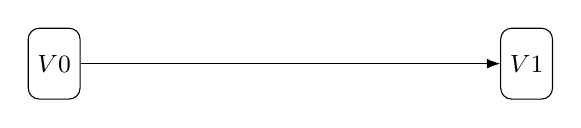
\begin{tikzpicture}[>=Latex,box/.style={draw,rounded corners,align=center,minimum height=9mm,font=\small},scale=1,transform shape]
\node[box] (v0) at (0,0) {$V0$};
\node[box] (v1) at (6,0) {$V1$};
\draw[->] (v0) -- (v1);
\end{tikzpicture}\end{center}

The arrow above denotes the erroneous forcing event.
To detect it, initialize the victim to 0,
initialize the aggressor to 0,
perform the aggressor transition and read the victim before any legitimate
write overwrites the corruption. The fault-free FSM leaves the victim unchanged.

(b) March C$-$ is
\[
\{\any(w0);\up(r0,w1);\up(r1,w0);
  \dn(r0,w1);\dn(r1,w0);\any(r0)\}.
\]
Use the six controller states below; two-operation states have read and write
subphases at each address.
\begin{center}\begin{tabular}{llll}\toprule State & Direction & Per-address operations & Next\\\midrule
$S_0$ & either & $w0$ & $S_1$\\
$S_1$ & up & $r0,w1$ & $S_2$\\
$S_2$ & up & $r1,w0$ & $S_3$\\
$S_3$ & down & $r0,w1$ & $S_4$\\
$S_4$ & down & $r1,w0$ & $S_5$\\
$S_5$ & either & $r0$ & Done\\\bottomrule
\end{tabular}\end{center}
Advance the address only after all operations of the current element finish.
At the last address, reload the appropriate end address and move to the next
state. Generate write data and expected read data from the state/subphase.
The total is $10N$ memory operations for $N$ addresses, ignoring setup cycles.

(c) A \emph{pattern/address generator} emits addresses, data and read/write
controls; a \emph{controller} sequences the March elements and handles timing;
a \emph{response analyzer} compares read data with expected data and records
pass/fail or failing addresses/bits. In a practical implementation, address and
data generation may be separate datapath blocks under that controller.

\section{Memory repair and reconfiguration}
\textbf{Question.} List three memory-reconfiguration mechanisms and compare
their advantages and disadvantages. Explain the functions of BIST,
diagnosis, redundancy analysis and reconfiguration in BISR.
\sol Examples of three practical mechanisms are:
\begin{center}\begin{tabular}{>{\raggedright\arraybackslash}p{28mm}>{\raggedright\arraybackslash}p{55mm}>{\raggedright\arraybackslash}p{55mm}}\toprule
Mechanism & Advantages & Limitations\\\midrule
Laser-programmed fuse links & Permanent setting; no boot-loading step &
Physical laser access and manufacturing equipment; ordinarily one-time\\
Electrically programmable fuses & On-chip programming; permanent repair
without laser access & Programming voltage/current and verification;
finite fuse resources and one-time choices\\
Volatile repair registers loaded at boot & Reconfigurable, easy to update
after a fresh test & Must be restored after power loss; requires boot-time
testing or a trusted nonvolatile repair map\\\bottomrule
\end{tabular}\end{center}
BIST applies tests and detects failures. Built-in self-diagnosis localizes
the failing addresses/bits or fault syndromes. The built-in redundancy analyzer
chooses spare rows/columns under a finite spare budget, or declares an
unrepairable map. Reconfiguration stores/loads that map and redirects accesses
to the spare resources. Finally, rerun tests to verify the repaired memory.
Detection alone does not calculate a valid spare assignment.

\section{Reading the fuse-bit circuit}
\textbf{Question.} A fuse bit has an active-low PMOS precharge control
FReset, an NMOS read control FRead, a fuse to ground with an FGND-controlled
bypass device, and a scan/update latch. Explain how to read fuse data at node $A$.
\begin{center}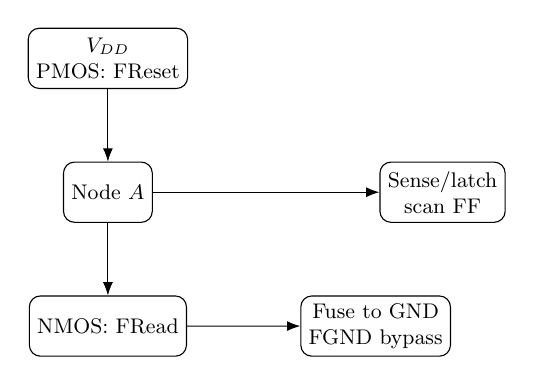
\begin{tikzpicture}[>=Latex,box/.style={draw,rounded corners,align=center,minimum height=9mm,font=\small},scale=0.85,transform shape]
\node[box] (pre) at (0,1) {$V_{DD}$\\PMOS: FReset};
\node[box] (a) at (0,-1) {Node $A$};
\node[box] (read) at (0,-3) {NMOS: FRead};
\node[box] (fuse) at (4,-3) {Fuse to GND\\FGND bypass};
\node[box] (latch) at (5,-1) {Sense/latch\\scan FF};
\draw[->] (pre) -- (a);
\draw[->] (a) -- (read);
\draw[->] (read) -- (fuse);
\draw[->] (a) -- (latch);
\end{tikzpicture}\end{center}

\sol Keep FRead=0 and the bypass FGND=0. Assert FReset=0 to precharge $A$ to 1.
Release FReset to 1, then pulse FRead=1 while FGND remains 0.
An intact fuse supplies a discharge path, making $A=0$; an open/blown fuse
leaves $A$ high. Allow settling, isolate the read path and capture the sensed
value in the scan flip-flop. In the drawn mux, Test\_Update=0 selects the
fuse-node path; Test\_Update=1 selects the scan value for a test override.
Do not enable the FGND bypass during sensing: it would discharge $A$
regardless of fuse continuity. Exact pulse widths and latch strength are
electrical implementation parameters not specified by this logic diagram.

\end{document}
